\documentclass[11pt,a4paper]{article}

% Packages (no application code listings; diagrams/tables/graphs only)
\usepackage[utf8]{inputenc}
\usepackage[T1]{fontenc}
\usepackage{lmodern}
\usepackage[margin=1in]{geometry}
\usepackage{hyperref}
\usepackage{xcolor}
\usepackage{graphicx}
\usepackage{amsmath}
\usepackage{booktabs}
\usepackage{tabularx}
\usepackage{enumitem}
\usepackage{fancyhdr}
\usepackage{tikz}
\usetikzlibrary{arrows.meta,positioning,shapes,fit,calc}
\usepackage{pgfplots}
\pgfplotsset{compat=1.18}
\usepackage{float}

% Hyperref setup
\hypersetup{
  colorlinks=true,
  linkcolor=blue,
  urlcolor=cyan
}

% Header/Footer
\pagestyle{fancy}
\fancyhf{}
\lhead{Data Ingestion \& Storage}
\rhead{BetterSys Architecture}
\rfoot{Page \thepage}

% Simple styles
\definecolor{bbblue}{RGB}{0,122,204}
\definecolor{bbgray}{RGB}{80,80,80}

% Make page layout more deterministic (helps keep the document to ~5 pages when compiled)
\setlength{\textfloatsep}{8pt plus 2pt minus 2pt}
\setlength{\floatsep}{6pt plus 2pt minus 2pt}
\setlength{\intextsep}{6pt plus 2pt minus 2pt}
\renewcommand{\arraystretch}{0.95}

\title{\textbf{BetterSys: Data Ingestion \& Storage}\\\large High-Level (No Code) System Overview}
\author{System Documentation}
\date{January 2026}

\begin{document}

\maketitle

\section*{1. System Overview (What data enters, what gets stored)}

BetterSys ingests multiple external market and wallet-activity streams, normalizes them into a unified \emph{signal} representation, persists durable records in SQLite, and serves low-latency reads to the terminal UI via REST + WebSocket.

\vspace{0.5em}
\noindent\textbf{Primary stored data products}
\begin{itemize}[leftmargin=*]
  \item \textbf{Signals:} compact, append-only records representing detected trading opportunities and tracked wallet actions.
  \item \textbf{Enrichment context:} per-signal, versioned context blobs (market metadata, entry price, orderbook snapshots, activity, derived metrics). For ultra-high-frequency 15m Up/Down signals, only a lite context is persisted.
  \item \textbf{Raw Dome order events:} lossless WebSocket payloads for auditability and downstream analytics.
  \item \textbf{Search index:} FTS5-backed full-history search records for robust terminal lookup.
  \item \textbf{DB-backed caches:} small JSON caches with TTLs (market metadata, wallet analytics, mapping) to keep endpoints responsive under upstream volatility.
\end{itemize}

\begin{figure}[H]
\centering
\begin{tikzpicture}[
  node distance=1.2cm,
  box/.style={rectangle, draw, rounded corners, minimum width=3.0cm, minimum height=0.9cm, align=center, font=\small},
  db/.style={cylinder, draw, shape border rotate=90, aspect=0.25, minimum height=1.0cm, minimum width=2.2cm, align=center, font=\small},
  arrow/.style={-Latex, thick},
  dash/.style={-Latex, thick, dashed}
]
  % External sources
  \node[box] (domews) {DomeAPI\\WebSocket\\(orders)};
  \node[box, right=of domews] (domerest) {DomeAPI\\REST\\(fallback + enrich)};
  \node[box, right=of domerest] (gamma) {Polymarket\\GAMMA\\(markets/events)};
  \node[box, right=of gamma] (hashdive) {Hashdive\\(whale trades)};
  \node[box, below=of gamma] (clob) {Polymarket CLOB\\(orderbook snapshots)};
  \node[box, below=of domews] (binance) {Binance\\(price feed)};

  % Ingestion / processing
  \node[box, below=1.5cm of domerest, minimum width=4.2cm] (ingest) {Ingestion Layer\\(pollers + WS handlers)};
  \node[box, right=of ingest, minimum width=4.2cm] (normalize) {Normalize \& Detect\\(signal construction)};
  \node[box, right=of normalize, minimum width=3.2cm] (quality) {Quality Gate\\(drop low-quality)};

  % Storage and serving
  \node[db, below=1.6cm of normalize] (sqlite) {SQLite\\(WAL mode)};
  \node[box, left=2.2cm of sqlite] (wsout) {WS Broadcast\\(signal + context)};
  \node[box, right=2.2cm of sqlite] (restout) {REST API\\(lists/search/context)};
  \node[box, below=of sqlite, minimum width=4.2cm] (frontend) {Terminal UI\\(REST hydrate + WS merge)};

  % Arrows in
  \draw[arrow] (domews) -- (ingest);
  \draw[dash] (domerest) -- (ingest);
  \draw[arrow] (gamma) -- (ingest);
  \draw[arrow] (hashdive) -- (ingest);
  \draw[arrow] (clob) -- (ingest);
  \draw[arrow] (binance) -- (ingest);

  % Pipeline
  \draw[arrow] (ingest) -- (normalize);
  \draw[arrow] (normalize) -- (quality);
  \draw[arrow] (quality) -- (sqlite);
  \draw[arrow] (quality) |- (wsout);
  \draw[arrow] (sqlite) -- (restout);
  \draw[arrow] (wsout) |- (frontend);
  \draw[arrow] (restout) |- (frontend);

  % Labels
  \node[font=\scriptsize, text=bbgray] at ($(domews)!0.5!(ingest)$) {real-time};
  \node[font=\scriptsize, text=bbgray] at ($(domerest)!0.5!(ingest)$) {fallback/enrich};
\end{tikzpicture}
\caption{End-to-end data flow: external sources \ensuremath{\rightarrow} ingestion \ensuremath{\rightarrow} signals \ensuremath{\rightarrow} SQLite \ensuremath{\rightarrow} REST/WS.}
\end{figure}

\vspace{-0.5em}
\begin{table}[H]
\centering
\small
\begin{tabularx}{\textwidth}{@{}l l l X@{}}
\toprule
\textbf{Source} & \textbf{Protocol} & \textbf{Cadence} & \textbf{Stored outcome (high-level)} \\
\midrule
DomeAPI Orders & WS & sub-second & Signals + raw order payloads; optional enrichment context \\
DomeAPI Orders & REST & periodic fallback & Same signal form; used to backfill and to enrich \\
Polymarket GAMMA & REST & batch polling & Market/event snapshots used to derive signals and metadata \\
Polymarket CLOB & REST/WS (on-demand) & triggered by UI/enrich & Orderbook snapshots cached + attached to context \\
Hashdive & REST & batch polling & Whale trade signals + attribution metadata \\
Binance & WS & real-time & Price snapshots (primarily for 15m engines and latency monitoring) \\
\bottomrule
\end{tabularx}
\caption{Key ingestion sources and what ultimately becomes durable.}
\end{table}

\newpage

\section*{2. Ingestion Layer: Cadence, resilience, and backpressure}

The ingestion layer runs multiple concurrent workers. Each worker has explicit timeouts and error accounting, and sources can be automatically disabled via a \emph{kill-switch} when they exceed failure or latency thresholds. The goal is to keep the overall pipeline responsive even when upstream providers intermittently return 5xx or slow responses.

\subsection*{2.1 Worker classes}
\begin{itemize}[leftmargin=*]
  \item \textbf{Streaming workers (WS):} receive events continuously (e.g., tracked wallet orders). Designed for minimal per-event work.
  \item \textbf{Polling workers (REST batch):} periodically fetch batches (e.g., market lists, whale trades). Designed for throughput and rate-limit friendliness.
  \item \textbf{On-demand fetchers:} triggered by UI tabs (book snapshots) or enrichment jobs; aggressively cached to avoid storms.
\end{itemize}

\subsection*{2.2 Fallback paths and supervisory controls}

\begin{figure}[H]
\centering
\begin{tikzpicture}[
  node distance=1.1cm,
  box/.style={rectangle, draw, rounded corners, minimum width=3.4cm, minimum height=0.9cm, align=center, font=\small},
  ctrl/.style={rectangle, draw, rounded corners, fill=bbblue!10, minimum width=3.4cm, minimum height=0.9cm, align=center, font=\small},
  arrow/.style={-Latex, thick},
  dash/.style={-Latex, thick, dashed}
]
  \node[box] (ws) {Dome WS\\Primary stream};
  \node[box, below=of ws] (restfb) {Dome REST\\Fallback poll};
  \node[ctrl, right=2.0cm of ws] (ks) {Kill-switch\\(failures + p95 latency)};
  \node[box, right=2.0cm of restfb] (queue) {Bounded work queues\\(detect + enrich)};
  \node[box, below=of queue] (workers) {Worker pool\\(rate-limited)};
  \node[box, below=of restfb] (persist) {SQLite writes\\(batch + upsert)};

  \draw[arrow] (ws) -- (queue);
  \draw[dash] (restfb) -- (queue);
  \draw[arrow] (ks) -- (ws);
  \draw[arrow] (ks) -- (restfb);
  \draw[arrow] (queue) -- (workers);
  \draw[arrow] (workers) -- (persist);

  \node[font=\scriptsize, text=bbgray] at ($(ws)!0.5!(queue)$) {fast path};
  \node[font=\scriptsize, text=bbgray] at ($(restfb)!0.5!(queue)$) {degraded mode};
\end{tikzpicture}
\caption{Resilience model: WS-first, REST fallback, supervisory kill-switch, bounded queues to prevent overload.}
\end{figure}

\subsection*{2.3 Typical latency/freshness trade-offs (conceptual)}

\begin{figure}[H]
\centering
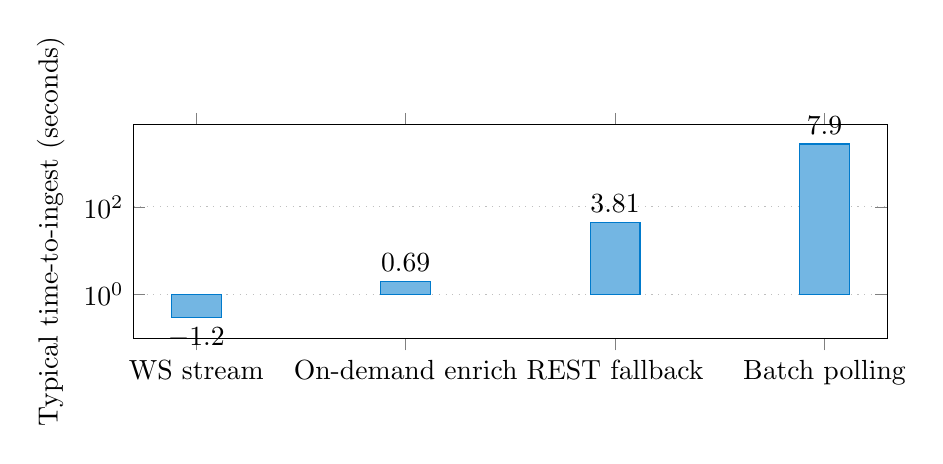
\begin{tikzpicture}
\begin{axis}[
  ybar,
  bar width=18pt,
  width=0.92\textwidth,
  height=4.3cm,
  ymode=log,
  ymin=0.1,
  ylabel={Typical time-to-ingest (seconds)},
  symbolic x coords={WS stream,On-demand enrich,REST fallback,Batch polling},
  xtick=data,
  x tick label style={align=center},
  nodes near coords,
  nodes near coords align={vertical},
  ymajorgrids=true,
  grid style={dotted,gray!50},
]
\addplot[fill=bbblue!55, draw=bbblue] coordinates {
  (WS stream,0.3)
  (On-demand enrich,2)
  (REST fallback,45)
  (Batch polling,2700)
};
\end{axis}
\end{tikzpicture}
\caption{Conceptual freshness: streaming is sub-second; enrichment is seconds; fallback polling is tens of seconds; batch polling is minutes.}
\end{figure}

\vspace{-0.8em}
\begin{table}[H]
\centering
\small
\begin{tabularx}{\textwidth}{@{}l l X X@{}}
\toprule
\textbf{Ingestion job} & \textbf{Trigger} & \textbf{Input} & \textbf{Primary durable writes} \\
\midrule
Tracked wallet stream & continuous & Dome WS order events & \emph{signals}, \emph{dome\_order\_events}; optional \emph{signal\_context} \\
REST fallback orders & periodic & Dome REST order history & \emph{signals} (dedup by stable IDs), optional context \\
Market batch polling & periodic & Gamma markets/events & \emph{signals} and cached metadata (\texttt{dome\_cache}) \\
Whale polling & periodic & Hashdive whale trades & \emph{signals} with attribution details \\
Search backfill & periodic & Stored signals & \emph{signal\_search} (+ FTS table via triggers) \\
Wallet analytics warm & periodic + on-demand & Dome pnl + local orderflow & \emph{dome\_cache} (analytics key + TTL) \\
Pruning/maintenance & periodic & SQLite tables & deletes/compaction for bounded growth (e.g., old raw events) \\
\bottomrule
\end{tabularx}
\caption{Ingestion and background jobs (conceptual naming; each maps to a dedicated worker loop).}
\end{table}

\newpage

\section*{3. Normalization \& Signal Lifecycle (from raw event to enriched, searchable record)}

All inputs are normalized into a compact \emph{signal} object with stable identity, timestamps, market identifiers, and a bounded details payload. Enrichment is asynchronous: signals are emitted immediately for latency, then context is attached later when available.

\subsection*{3.1 Identity, deduplication, and idempotency}
\begin{itemize}[leftmargin=*]
  \item \textbf{Stable signal IDs} are derived from upstream event identity (e.g., an order hash). This allows deterministic joins between the initial signal and later context updates.
  \item \textbf{Deduplication} is performed at storage boundaries using the signal ID as a primary key (insert-or-ignore/upsert patterns).
  \item \textbf{Versioned context} uses a monotonically increasing \emph{context version} per signal, enabling safe last-write-wins merges in the UI.
\end{itemize}

\subsection*{3.2 Real-time path: tracked wallet order \ensuremath{\rightarrow} signal \ensuremath{\rightarrow} context update}

\begin{figure}[H]
\centering
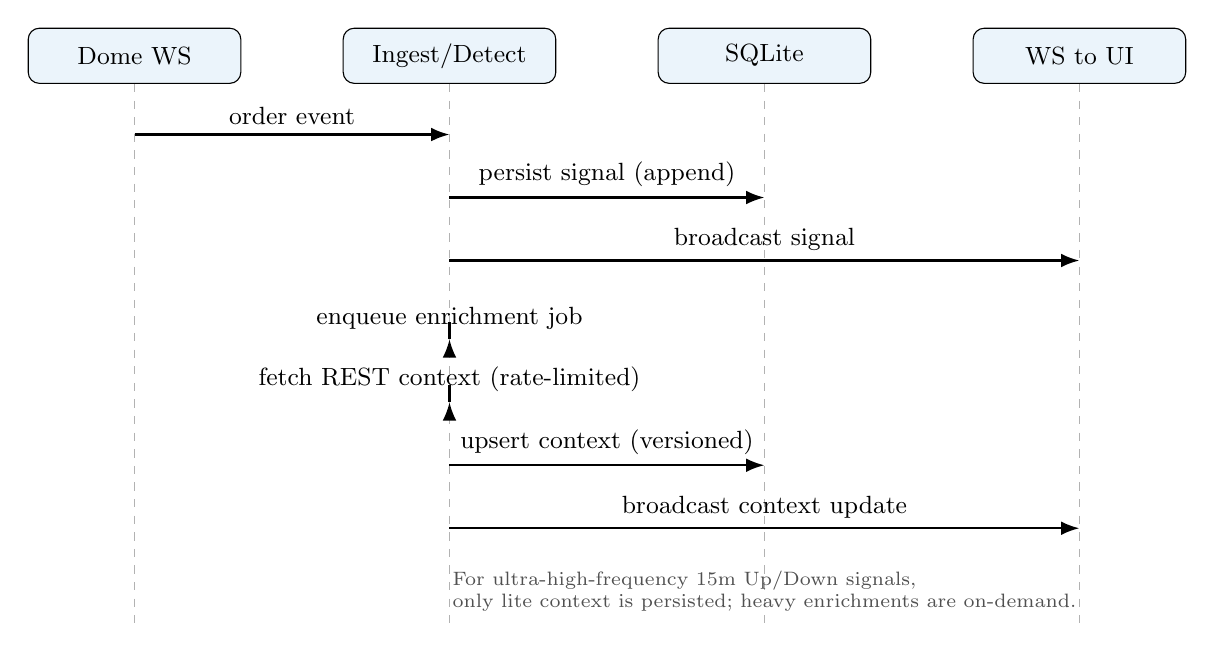
\begin{tikzpicture}[
  font=\small,
  lifeline/.style={draw, dashed, gray!60},
  actor/.style={rectangle, draw, rounded corners, fill=bbblue!8, minimum width=2.7cm, minimum height=0.7cm, align=center},
  msg/.style={-Latex, thick},
]
  % Actors
  \node[actor] (a1) at (0,0) {Dome WS};
  \node[actor] (a2) at (4.0,0) {Ingest/Detect};
  \node[actor] (a3) at (8.0,0) {SQLite};
  \node[actor] (a4) at (12.0,0) {WS to UI};

  % Lifelines
  \draw[lifeline] (a1.south) -- (0,-7.2);
  \draw[lifeline] (a2.south) -- (4,-7.2);
  \draw[lifeline] (a3.south) -- (8,-7.2);
  \draw[lifeline] (a4.south) -- (12,-7.2);

  % Messages
  \draw[msg] (0,-1.0) -- node[above]{order event} (4,-1.0);
  \draw[msg] (4,-1.8) -- node[above]{persist signal (append)} (8,-1.8);
  \draw[msg] (4,-2.6) -- node[above]{broadcast signal} (12,-2.6);

  % Enrichment branch
  \draw[msg] (4,-3.6) -- node[above]{enqueue enrichment job} (4.0,-3.6);
  \draw[msg] (4,-4.4) -- node[above]{fetch REST context (rate-limited)} (4.0,-4.4);
  \draw[msg] (4,-5.2) -- node[above]{upsert context (versioned)} (8,-5.2);
  \draw[msg] (4,-6.0) -- node[above]{broadcast context update} (12,-6.0);

  % Notes
  \node[align=left, font=\scriptsize, text=bbgray] at (8.0,-6.8) {For ultra-high-frequency 15m Up/Down signals,\\only lite context is persisted; heavy enrichments are on-demand.};
\end{tikzpicture}
\caption{Sequence (conceptual): signal is emitted immediately; enrichment is asynchronous and versioned.}
\end{figure}

\subsection*{3.3 Lifecycle states}

\begin{table}[H]
\centering
\small
\begin{tabularx}{\textwidth}{@{}l l X X@{}}
\toprule
\textbf{Stage} & \textbf{Storage} & \textbf{What is guaranteed} & \textbf{Why it exists} \\
\midrule
Raw event received & dome\_order\_events (WS only) & Lossless payload capture (audit trail) & Debugging, analytics, reconstruction \\
Signal persisted & signals & Durable, compact record with stable ID & Fast lists, pagination, de-dupe anchor \\
Context attached & signal\_context & Best-effort enrichment; versioned upserts & Rich UI, explainability, debugging \\
Searchable record & signal\_search + FTS & Full-history lookup; incremental backfill & Terminal search beyond in-memory window \\
Cached heavy results & dome\_cache & TTL-bounded JSON snapshots & Speed + resilience under upstream failures \\
\bottomrule
\end{tabularx}
\caption{Signal lifecycle and how it maps to durable storage (table names reflect the SQLite schema).}
\end{table}

\newpage

\section*{4. Storage Design (SQLite): schemas, indexing, caching, and retention}

BetterSys uses SQLite (WAL mode) as the primary durable store for signals and related artifacts. WAL enables concurrent reads during writes, and the write path is optimized via batching and careful indexing.

\subsection*{4.1 Database partitioning (separation of concerns)}
\begin{itemize}[leftmargin=*]
  \item \textbf{Signals DB:} signal records, enrichment context, search index, raw Dome events, and TTL caches.
  \item \textbf{Auth DB:} users/sessions for API authentication.
  \item \textbf{Vault DB:} pooled-vault accounting state (shares/NAV) in a separate file to reduce coupling.
\end{itemize}

\subsection*{4.2 Logical schema (high-level)}

\begin{figure}[H]
\centering
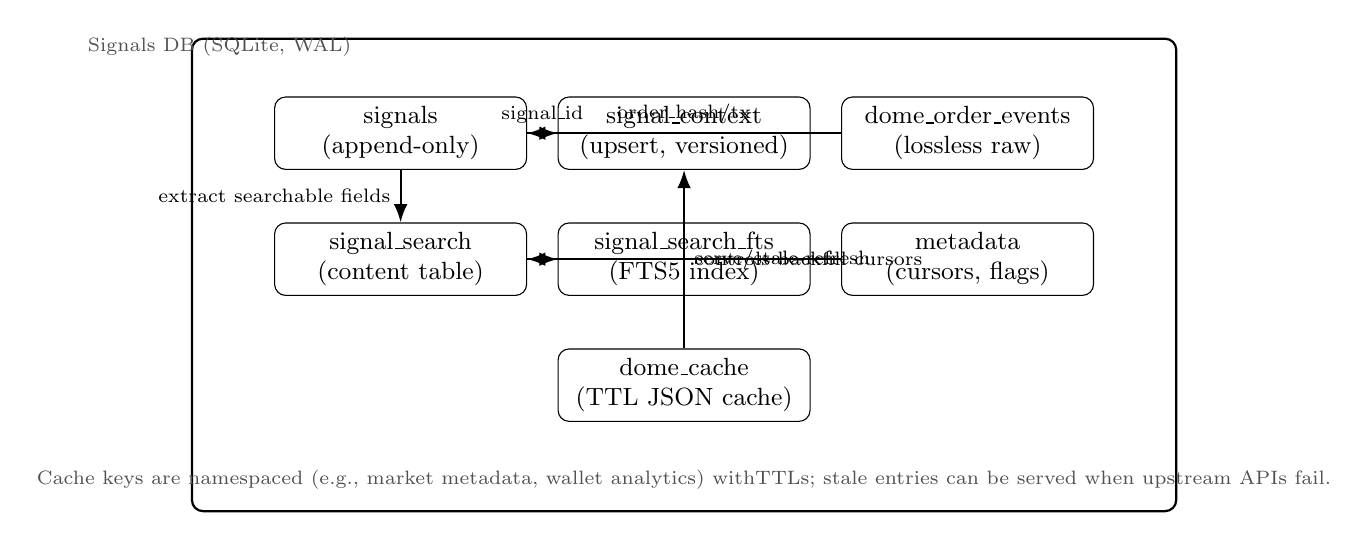
\begin{tikzpicture}[
  box/.style={rectangle, draw, rounded corners, minimum width=3.2cm, minimum height=0.9cm, align=center, font=\small},
  db/.style={rectangle, draw, thick, rounded corners, minimum width=12.5cm, minimum height=6.0cm},
  arrow/.style={-Latex, thick},
  note/.style={font=\scriptsize, text=bbgray, align=left}
]
  \node[db] (signalsdb) at (0,0) {};
  \node[note] at (-5.9,2.9) {Signals DB (SQLite, WAL)};

  \node[box] (signals) at (-3.6,1.8) {signals\\(append-only)};
  \node[box] (ctx) at (0.0,1.8) {signal\_context\\(upsert, versioned)};
  \node[box] (raw) at (3.6,1.8) {dome\_order\_events\\(lossless raw)};

  \node[box] (search) at (-3.6,0.2) {signal\_search\\(content table)};
  \node[box] (fts) at (0.0,0.2) {signal\_search\_fts\\(FTS5 index)};
  \node[box] (meta) at (3.6,0.2) {metadata\\(cursors, flags)};

  \node[box] (cache) at (0.0,-1.4) {dome\_cache\\(TTL JSON cache)};

  \draw[arrow] (signals) -- node[above, font=\scriptsize]{signal\_id} (ctx);
  \draw[arrow] (raw) -- node[above, font=\scriptsize]{order\_hash/tx} (signals);
  \draw[arrow] (search) -- (fts);
  \draw[arrow] (signals) -- node[left, font=\scriptsize]{extract searchable fields} (search);
  \draw[arrow] (meta) -- node[right, font=\scriptsize]{controls backfill cursors} (search);
  \draw[arrow] (cache) -- node[right, font=\scriptsize]{serve/stale-refresh} (ctx);

  \node[note] at (0.0,-2.6) {Cache keys are namespaced (e.g., market metadata, wallet analytics) with\newline TTLs; stale entries can be served when upstream APIs fail.};
\end{tikzpicture}
\caption{High-level storage relationships inside the signals SQLite database.}
\end{figure}

\subsection*{4.3 Table inventory (what is stored and how it grows)}

\begin{table}[H]
\centering
\small
\begin{tabularx}{\textwidth}{@{}l l l X@{}}
\toprule
\textbf{Table} & \textbf{Growth} & \textbf{Key} & \textbf{Contents (summary)} \\
\midrule
signals & unbounded (append) & signal\_id & Compact signal facts (type, market slug, confidence, timestamps, source) \\
signal\_context & bounded by signals & signal\_id & Versioned per-signal context blob; may be partial/failed \\
dome\_order\_events & pruned (retention) & order\_hash & Lossless Dome WS payloads + minimal indexing fields \\
signal\_search & backfilled & signal\_id & Search-friendly columns derived from signals/context \\
signal\_search\_fts & mirrors search & rowid & Full-text index for robust terminal search \\
metadata & tiny & key & Cursors, backfill state, feature flags, schema markers \\
dome\_cache & bounded by TTL & cache\_key & JSON snapshots (market metadata, analytics, mappings) with fetched timestamps \\
\bottomrule
\end{tabularx}
\caption{SQLite tables and their growth model (append-only vs TTL vs pruning).}
\end{table}

\subsection*{4.4 Storage growth control (conceptual)}

\begin{figure}[H]
\centering
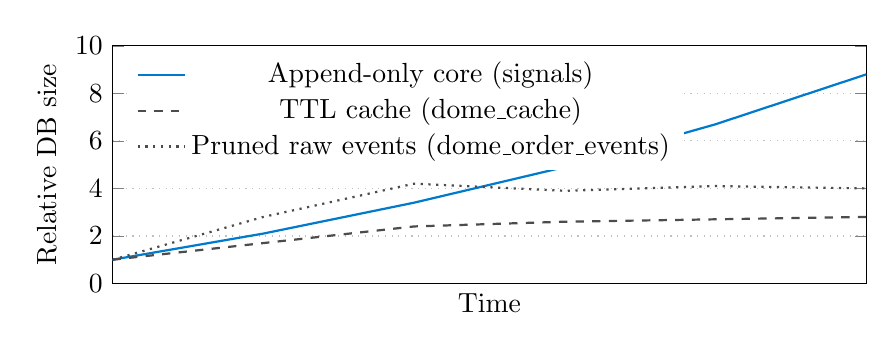
\begin{tikzpicture}
\begin{axis}[
  width=0.92\textwidth,
  height=4.6cm,
  xlabel={Time},
  ylabel={Relative DB size},
  xmin=0,xmax=10,
  ymin=0,ymax=10,
  xtick=\empty,
  ymajorgrids=true,
  grid style={dotted,gray!50},
  legend style={at={(0.02,0.98)},anchor=north west,draw=none,fill=white},
]
\addplot[thick, bbblue] coordinates {(0,1) (2,2.1) (4,3.4) (6,4.9) (8,6.7) (10,8.8)};
\addlegendentry{Append-only core (signals)}
\addplot[thick, dashed, color=black!70] coordinates {(0,1) (2,1.7) (4,2.4) (6,2.6) (8,2.7) (10,2.8)};
\addlegendentry{TTL cache (dome\_cache)}
\addplot[thick, dotted, color=black!70] coordinates {(0,1) (2,2.8) (4,4.2) (6,3.9) (8,4.1) (10,4.0)};
\addlegendentry{Pruned raw events (dome\_order\_events)}
\end{axis}
\end{tikzpicture}
\caption{Conceptual growth: signals are append-only; caches are TTL-bounded; raw WS payloads are pruned by retention policy.}
\end{figure}

\newpage

\section*{5. Serving layer: query patterns, search, and consistency guarantees}

The system is optimized for a terminal UX: recent signals must load quickly, full-history search must be responsive, and UI panels must avoid ``infinite loading'' even during upstream instability.

\subsection*{5.1 Read paths and caching layers}

\begin{figure}[H]
\centering
\begin{tikzpicture}[
  box/.style={rectangle, draw, rounded corners, minimum width=3.4cm, minimum height=0.9cm, align=center, font=\small},
  db/.style={cylinder, draw, shape border rotate=90, aspect=0.25, minimum height=1.0cm, minimum width=2.2cm, align=center, font=\small},
  arrow/.style={-Latex, thick},
  dash/.style={-Latex, thick, dashed}
]
  \node[box] (ui) {Terminal UI};
  \node[box, right=2.0cm of ui] (api) {REST API};
  \node[box, below=of api] (ws) {WebSocket};
  \node[db, right=2.0cm of api] (db) {SQLite};
  \node[box, below=of db] (cache) {DB-backed cache\\(TTL + stale fallback)};

  \draw[arrow] (ui) -- node[above, font=\scriptsize]{lists / search / context} (api);
  \draw[arrow] (api) -- (db);
  \draw[arrow] (ui) -- node[left, font=\scriptsize]{real-time updates} (ws);
  \draw[arrow] (ws) -- (ui);
  \draw[dash] (api) -- node[right, font=\scriptsize]{analytics / enrich} (cache);
  \draw[arrow] (cache) -- (db);

  \node[font=\scriptsize, text=bbgray, align=left] at ($(ui)+(0,-2.5)$) {UI strategy: REST hydrates a recent window; WS streams new events;\newline search uses FTS5; heavy panels use cache + timeouts to avoid stalls.};
\end{tikzpicture}
\caption{Serving layer: REST + WS backed by SQLite; heavy reads use TTL cache with stale fallback.}
\end{figure}

\subsection*{5.2 Endpoint-to-storage mapping (conceptual)}

\begin{table}[H]
\centering
\small
\begin{tabularx}{\textwidth}{@{}l X X@{}}
\toprule
\textbf{User-facing capability} & \textbf{Primary store} & \textbf{Notes (reliability/latency)} \\
\midrule
Recent signals list + pagination & signals (+ lite context) & Designed for fast scans with covering indexes; bounded payloads \\
Per-signal context fetch & signal\_context & Versioned; can return partial/failed status without blocking the UI \\
Full-history search & signal\_search\_fts & Warm-up indexing + incremental backfill ensures search is never ``dead'' \\
Wallet analytics curves & dome\_cache & TTL 15m; SWR pattern: serve cached quickly, refresh in background \\
Orderbook snapshot panels & dome\_cache + on-demand fetch & Rate-limited; cached to prevent request storms; may serve stale when upstream fails \\
\bottomrule
\end{tabularx}
\caption{How terminal features map to SQLite tables and caches.}
\end{table}

\subsection*{5.3 Consistency model (what to expect)}
\begin{itemize}[leftmargin=*]
  \item \textbf{Signals are durable and monotonic by time:} once a signal is stored, it is never mutated (only additional context may be attached).
  \item \textbf{Context is eventually consistent:} enrichment may arrive later, partially, or not at all; the UI treats context as a best-effort add-on.
  \item \textbf{Search is convergent:} recent signals are indexed early; deep history is backfilled incrementally with cursor state stored in metadata.
  \item \textbf{Fail-open under upstream instability:} when external APIs return 5xx or time out, cached values (possibly stale) are served to prevent blank panels.
\end{itemize}

\subsection*{5.4 Operational checklist (data integrity focused)}
\begin{enumerate}[leftmargin=*]
  \item Use WAL mode for concurrent readers while writers batch commits.
  \item Keep raw-event retention bounded (prune old \texttt{dome\_order\_events}) to cap disk growth.
  \item Treat caches as disposable: correctness comes from \texttt{signals} + upstream re-fetch, not from cached JSON.
  \item Ensure enrichment and search backfill are rate-limited and queue-bounded to avoid tail-latency spikes.
\end{enumerate}

\vfill
\noindent\textbf{End state:} a resilient ingestion-and-storage pipeline that prioritizes real-time signal delivery, durable audit trails, bounded payload sizes, and fast terminal queries.

\end{document}
